\begin{frame}{Espaces m\'etriques}
\begin{definition}
Un espace m\'etrique d\'enombrable discret  $X$ est \`a \textit{g\'eom\'etrie born\'ee} si
\[\sup_{x\in X} | B(x,r)| < \infty \quad \forall r >0.\]
\end{definition}
\textit{Exemples typiques}\\
\vfill
\begin{itemize}
\item[$\bullet$] $X=(V,E)$ graphe de degr\'e uniform\'ement born\'e.
\vfill
\item[$\bullet$] $G=\langle S \rangle$ groupe finiement engendr\'e, muni de la \textit{m\'etrique des mots}\\
\[l(g) = \inf\{k : g = s_1 s_2 ... s_k , \ s_i \in S\}, \quad d(g,h) = l(g^{-1}h).\]
\end{itemize}
\vfill
footnote  $e_G\notin S$ et $S=S^{-1}$
\end{frame}

\begin{frame}{Graphe de Cayley}
La m\'etrique des mots peut \^{e}tre r\'ealis\'ee comme une distance de graphe.\\
\vfill
\begin{definition}
Le \textit{Graphe de Cayley} associ\'ee au couple $(G,S)$ est 
\[|G| = (V,E_S)\]
avec : 
\vfill
\begin{itemize}
\item[$\bullet$] $V=G$,
\vfill
\item[$\bullet$] $(x,y)\in E_S$ ssi $x^{-1}y\in S$.
\end{itemize}
\end{definition}
\vfill
\end{frame}

\begin{frame}{$G=\Z$}
\[S= \{\pm 1\}\]
\begin{tikzpicture}
\scriptsize
\newcount\N;
\N 4; 

\foreach \i in {-6,...,\N}
	{
	\draw (\i+1,0) node{$\bullet$};
	\draw (\i+1,0) node[below]{$\i$};
     \draw (\i,0) -- (\i+ 1,0);
	}
 	\draw (\N+1,0) -- (\N+2,0);
 
 \foreach \i in {-3,...,\N/2}
		{
		\draw (2*\i+1,-3) node{$\bullet$};
		\draw (2*\i,-4) node{$\bullet$};
     		\draw (2*\i,-4) -- (2*\i+2,-4);
	 	\draw (2*\i,-4) -- (2*\i+3,-3);
	  	\draw (2*\i+1,-3) -- (2*\i+4,-4);
	 	\draw (2*\i+1,-3) -- (2*\i+3,-3);
	 	}
	 	\draw (-5,-3) -- (-6,-3);
	 	\draw (-4,-4) -- (-6,-3.3);
	 	\draw (-5,-3) -- (-6,-3.3);
 		 
\draw (-5,-3) node[above]{-5};
\draw (-3,-3) node[above]{-3};
\draw (-1,-3) node[above]{-1};
\draw (1,-3) node[above]{1};
\draw (5,-3) node[above]{5};
\draw (3,-3) node[above]{3};

\draw (0,-4) node[below]{0};
\draw (2,-4) node[below]{2};
\draw (-2,-4) node[below]{-2};
\draw (4,-4) node[below]{4};
\draw (-4,-4) node[below]{-4};
\draw (-6,-4) node[below]{-6};
\end{tikzpicture}
\[S= \{\pm 2 , \pm 3\}\]
\end{frame}

%\begin{frame}{$G=\mathbb F_2$}
%\begin{picture}(8.5cm,8.5cm)(-4.2cm,-4.2cm)
%\linethickness{1.5pt}
%{\A}
%{\B}
%{\C}
%{\D}
%\end{picture}
%\end{frame}

\begin{frame}{$G=\mathbb F_2$}
\begin{center}
\begin{tikzpicture}
\draw (0,0) node{$\bullet$};
\foreach \i in {1,...,4}
{
	\draw (90*\i:2) node{$\bullet$};
      \draw (0,0) -- (90*\i: 2);      
}
\foreach \i in {1,...,4}
{\foreach \a in {-1,...,1}
{
	\draw (90*\i:2)+(90*\a+90*\i:1) node{$\bullet$};
      %\draw (0,0) -- (90*\i: 1);      
}}
\end{tikzpicture}
\end{center}
\end{frame}

\begin{frame}
\begin{center}
\vfill
\includegraphics[width=0.8\linewidth]{Cayley_2}
\vfill
\end{center}
\end{frame}

\begin{frame}
\begin{center}
\vfill
\includegraphics[width=0.8\linewidth]{Cayley}
\vfill
\end{center}
\end{frame}

\begin{frame}{$G=PSL(2,\Z)$}
\begin{center}
\begin{tikzpicture}
\scriptsize 
\foreach \i in {1,...,3}
{
	\draw (120*\i:1) node{$\bullet$};
      \draw (120* \i : 1) -- (120*\i+120: 1);
	\draw (120* \i : 1) -- (120*\i: 2);
      
}

\foreach \j in {1,...,3}
{\foreach \i in {1,...,3}
{
	\draw (120*\j:3)+(120*\i+60:1) node{$\bullet$};
	\draw  (120*\j:3)+(120*\i+60:1) -- (120*\j:3)+(120*\i+180:1) -- (120*\j:3)+(120*\i+300:1) -- cycle;
      %\draw ((120*\j:3)+(120*\i+60:1)) -- ((120*\j:3)+(120*\i+180:1));
}}
 
\end{tikzpicture}
\end{center}\end{frame}

\begin{frame}{Alg\`ebres de Roe}
Rappel: 
\[l^2X = Vect_{\mathbb C} \{e_x\}_{x\in X} \quad \langle e_x, e_y\rangle =\delta_{xy}. \]
est un espace de Hilbert. La norme est $\|x\| =\sqrt{\langle x, x\rangle}$.\\
\vfill
$B(l^2X)$ d\'enote l'alg\`ebre des op\'erateurs lin\'eaires born\'es. La norme
\[\|a\| = \sup \{ ||ax|| \ | \ \|x\| \leq 1 \} \] 
la munit d'une structure d'alg\`ebre de Banach.\\
\vfill
Pour $a\in B(l^2 X)$, on peut regarder les coefficients \[a_{xy} = \langle e_y, ae_x \rangle.\]
\end{frame}

\begin{frame}{Propagation finie}
On regarde \[\C_r [X] = \{ (a_{xy})\in B(l^2 X) \ : \ a_{xy }=0 \text{ si } d(x,y)> r\}  \]
Et \[\C_u[X] = \cup_{r>0} \C_r[X] \subset B(l^2 X) \]
est la sous-alg\'ebre de $B(l^2 X)$ des op\'erateurs de propagation finie.
\vfill
\end{frame}

\begin{frame}{Propagation finie}
\begin{center}%\vspace{0.5cm}
\vfill
\includegraphics[width=0.8\linewidth]{finite_propagation}
\vfill
%\captionof{figure}{\color{Green} A family of graphs}
\end{center}%\vspace{0.5cm}
\end{frame}

\begin{frame}{Alg\`ebre de Roe}
\begin{definition}
La compl\'etion de $\C_u[X]$ pour la norme d'op\'erateurs est appel\'ee \textit{l'alg\`ebre de Roe} de $X$. 
\end{definition}
\vfill
On la note $C^*_u(X)$.\\
\vfill
Int\'er\^{e}t: 
\begin{itemize}
\item[$\bullet$] th\'eor\`emes de l'indice \`a la Atiyah-Singer,
\item[$\bullet$] conjecture de Novikov,
\item[$\bullet$] conjecture de Baum-Connes.
\end{itemize}
\end{frame}

\begin{frame}{$K$-th\'eorie}
Donner un moyen de calculer les groupes de $K$-th\'eorie de $C^*_u(X)$.\\
\vfill
La $K$-th\'eorie d'une alg\`ebre de Banach $A$ est la donn\'ee de deux groupes ab\'eliens $K_0(A)$ et $K_1(A)$ qui sont des \'equivalents alg\'ebriques des groupes de cohomologie pour une vari\'et\'e par exemple.  
\vfill
R\^{o}le en classification.\\
\vfill

\end{frame}

\begin{frame}{$K$-th\'eorie}
Soit $H$ un espce de Hilbert s\'eparable.
\vfill
\begin{theorem}
Les sous-alg\'ebres ferm\'ees $A$ de $B(H)$ qui sont
\begin{itemize}
\item[$\bullet$] approximables par des alg\'ebres de matrices (\textit{nucl\'eaires}),
\item[$\bullet$] simples,
\item[$\bullet$] r\'eguli\`eres (au sens d'une dimension finie),
\item[$\bullet$] satisfont le th\'eor\`eme dit UCT ,
\end{itemize}
sont classifi\'ees par des invariant provenant de la $K$-th\'eorie.
\end{theorem} 
\vfill
\'Eliminer l'hypoth\`ese UCT est connue comme le \textit{probl\`eme UCT}. 
\end{frame}

\begin{frame}{Probl\`eme UCT pour $C^*_u(\Z)$}
Pour $R$ tr\`es grand,
\begin{center}
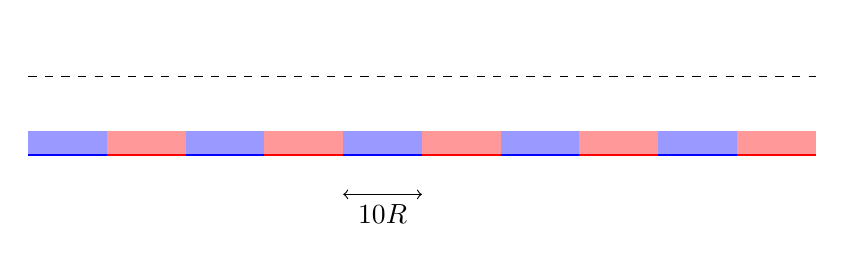
\begin{tikzpicture}
\draw (4.5,1.5) node{$\Z$};
\draw[dashed] (0,1)--(10,1);
\foreach \i in {0,...,4}
	{
	\fill[blue!40!white](2*\i,0) rectangle (2*\i+1,0.3);
	\draw[blue] (2*\i,0) -- (2*\i+1,0);
	}
\foreach \i in {0,...,4}
	{
	\fill[red!40!white](2*\i+1,0) rectangle (2*\i+2,0.3);
	\draw[red] (2*\i+1,0) -- (2*\i+2,0);
	}
\draw[<->] (4,-0.5) -- (5,-0.5);
\draw (4.5,-0.5) node[below]{$10R$};
\end{tikzpicture}
\end{center}
\end{frame}


